%%%%%%%%%%%%%%%%%%%%%%%%%%%%%%%%%%%%%%%%%%%%%%%%%%%%%%%%%%%%%%%%%%%%%%%%%%%%%%%%%%%%%%%%%%%%%%%%%%%%%%%%%%%%%%%%%%%%%%%%%%%%%%%%%%%%%%%%%%%%%%%%%%%%%%%%%%%%%%%%%%%
% Written By Michael Brodskiy
% Class: Circuits & Signals: Biomedical Applications
% Professor: N. Sun
%%%%%%%%%%%%%%%%%%%%%%%%%%%%%%%%%%%%%%%%%%%%%%%%%%%%%%%%%%%%%%%%%%%%%%%%%%%%%%%%%%%%%%%%%%%%%%%%%%%%%%%%%%%%%%%%%%%%%%%%%%%%%%%%%%%%%%%%%%%%%%%%%%%%%%%%%%%%%%%%%%%

\include{Includes.tex}

\title{Circuit Laws}
\date{\today}
\author{Michael Brodskiy\\ \small Professor: N. Sun}

\begin{document}

\maketitle

\begin{itemize}

  \item Voltmeter — Measures voltage without drawing current

  \item Ammeter — Measures current without dropping voltage

  \item Resistance is a function of size, shape, and media properties:

    $$\boxed{R=\frac{V}{I}=\frac{l}{\sigma A}=\rho\frac{l}{A}}$$

    \begin{itemize}

      \item $\sigma$ is the conductivity, $\rho$ is the resistivity, $l$ is the length of the wire, and $A$ is the cross-sectional area

    \end{itemize}

  \item Siemens (S), the unit for conductance, is the inverse of resistance, where: $\boxed{S=\dfrac{1}{\Omega}}$

    \begin{figure}[h!]
      \centering
      \tikzset{every picture/.style={line width=0.75pt}} %set default line width to 0.75pt        

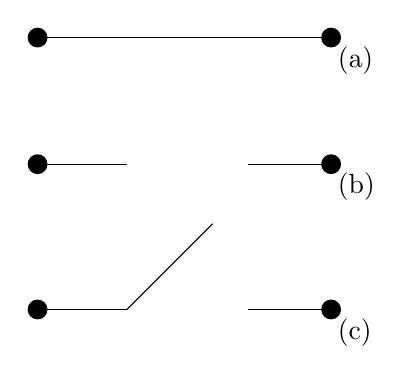
\begin{tikzpicture}[x=0.75pt,y=0.75pt,yscale=-1,xscale=1]
%uncomment if require: \path (0,359); %set diagram left start at 0, and has height of 359

%Shape: Boxed Line [id:dp6814534710440301] 
\draw    (399.71,51) -- (258.29,51) ;
%Shape: Circle [id:dp916629887844314] 
\draw  [fill={rgb, 255:red, 0; green, 0; blue, 0 }  ,fill opacity=1 ] (262.79,51) .. controls (262.79,48.51) and (260.77,46.5) .. (258.29,46.5) .. controls (255.8,46.5) and (253.79,48.51) .. (253.79,51) .. controls (253.79,53.49) and (255.8,55.5) .. (258.29,55.5) .. controls (260.77,55.5) and (262.79,53.49) .. (262.79,51) -- cycle ;
%Shape: Circle [id:dp26516064705603304] 
\draw  [fill={rgb, 255:red, 0; green, 0; blue, 0 }  ,fill opacity=1 ] (404.21,51) .. controls (404.21,48.51) and (402.2,46.5) .. (399.71,46.5) .. controls (397.23,46.5) and (395.21,48.51) .. (395.21,51) .. controls (395.21,53.49) and (397.23,55.5) .. (399.71,55.5) .. controls (402.2,55.5) and (404.21,53.49) .. (404.21,51) -- cycle ;
%Shape: Boxed Line [id:dp10516732114391769] 
\draw    (399.71,112) -- (258.29,112) ;
%Shape: Circle [id:dp05809513039601466] 
\draw  [fill={rgb, 255:red, 0; green, 0; blue, 0 }  ,fill opacity=1 ] (262.79,112) .. controls (262.79,109.51) and (260.77,107.5) .. (258.29,107.5) .. controls (255.8,107.5) and (253.79,109.51) .. (253.79,112) .. controls (253.79,114.49) and (255.8,116.5) .. (258.29,116.5) .. controls (260.77,116.5) and (262.79,114.49) .. (262.79,112) -- cycle ;
%Shape: Circle [id:dp7509947812401938] 
\draw  [fill={rgb, 255:red, 0; green, 0; blue, 0 }  ,fill opacity=1 ] (404.21,112) .. controls (404.21,109.51) and (402.2,107.5) .. (399.71,107.5) .. controls (397.23,107.5) and (395.21,109.51) .. (395.21,112) .. controls (395.21,114.49) and (397.23,116.5) .. (399.71,116.5) .. controls (402.2,116.5) and (404.21,114.49) .. (404.21,112) -- cycle ;
%Straight Lines [id:da01088402519767695] 
\draw [color={rgb, 255:red, 255; green, 255; blue, 255 }  ,draw opacity=1 ][fill={rgb, 255:red, 255; green, 255; blue, 255 }  ,fill opacity=1 ]   (301.29,112) -- (359.71,112) ;
%Shape: Boxed Line [id:dp9035438017815973] 
\draw    (399.71,182) -- (258.29,182) ;
%Shape: Circle [id:dp6675627274341545] 
\draw  [fill={rgb, 255:red, 0; green, 0; blue, 0 }  ,fill opacity=1 ] (262.79,182) .. controls (262.79,179.51) and (260.77,177.5) .. (258.29,177.5) .. controls (255.8,177.5) and (253.79,179.51) .. (253.79,182) .. controls (253.79,184.49) and (255.8,186.5) .. (258.29,186.5) .. controls (260.77,186.5) and (262.79,184.49) .. (262.79,182) -- cycle ;
%Shape: Circle [id:dp4832675708977021] 
\draw  [fill={rgb, 255:red, 0; green, 0; blue, 0 }  ,fill opacity=1 ] (404.21,182) .. controls (404.21,179.51) and (402.2,177.5) .. (399.71,177.5) .. controls (397.23,177.5) and (395.21,179.51) .. (395.21,182) .. controls (395.21,184.49) and (397.23,186.5) .. (399.71,186.5) .. controls (402.2,186.5) and (404.21,184.49) .. (404.21,182) -- cycle ;
%Straight Lines [id:da03336677807845523] 
\draw [color={rgb, 255:red, 255; green, 255; blue, 255 }  ,draw opacity=1 ][fill={rgb, 255:red, 255; green, 255; blue, 255 }  ,fill opacity=1 ]   (301.29,182) -- (359.71,182) ;
%Straight Lines [id:da0748980120101892] 
\draw [color={rgb, 255:red, 0; green, 0; blue, 0 }  ,draw opacity=1 ][fill={rgb, 255:red, 0; green, 0; blue, 0 }  ,fill opacity=1 ]   (301.29,182) -- (342.6,140.69) ;

% Text Node
\draw (401.71,54) node [anchor=north west][inner sep=0.75pt]   [align=left] {(a)};
% Text Node
\draw (401.71,115) node [anchor=north west][inner sep=0.75pt]   [align=left] {(b)};
% Text Node
\draw (401.71,185) node [anchor=north west][inner sep=0.75pt]   [align=left] {(c)};


\end{tikzpicture}

      \caption{Different Circuit Types}
      \label{fig:1}
    \end{figure}

    \begin{itemize}

      \item (a) shows a short circuit

      \item (b) shows an open circuit

      \item (c) shows an open switch

    \end{itemize}

  \item Kirchoff's Laws

    \begin{itemize}

      \item A circuit is said to be solved when voltage and current across each circuit element has been determined

      \item Consist of Kirchoff's current law (KCL) and Kirchoff's voltage law (KVL)

      \item Node — A point where two or more circuit elements meet

      \item Sum of currents entering a node is zero (also holds for closed boundary)

        $$\boxed{\sum_{n=1}^N i_n=0\,\,\,\,\,\,\,\,\text{(KCL)}}$$

      \item For any node, a unique voltage can be assigned

    \end{itemize}

\end{itemize}

\end{document}

